%-------------------------------------------------------------------
\section{Numerical Examples} \label{sec:ch5:examples}

In this section, we will use five numerical examples to demonstrate the efficacy of the proposed \apgp.
The first four examples have known solutions that can be used to compute the optimal trajectories and objective function value to high precision.
Therefore, we can directly compare the different solution methods based on their deviation from the known solution.
The errors are reported as local maximum/minimum values (i.e.,~as a forward-looking moving maximum/minimum) in order to discuss the converge behavior independent of fortuitous meshes (e.g.,~the nodes points happen to be exactly at the time value where a path constraint should change activity).
In addition to comparing the absolute error, we will look at the time to create the \qp{} with the \apgp{} and the total \qp{} time (creation plus solver time).
Other performance metrics include local and global error, robustness to initial guess\footnote{The chosen solver does not require an initial guess.}, and problem size or memory needed \cite{Williams2005a, Wang2009a}.
Please see Refs.~\cite{Williams2005a, Wang2009a, Faedo2017a} for numerical comparisons between some of the \dt{} methods.
It remains future work to perform these additional comparisons.

% new paragraph
All tests were performed on a personal computer with an i7-6800K at 3.8 GHz (up to 12 threads available), 32 GB DDR4 3200 MHz RAM, \textsc{Windows} 10 64-bit, and \textsc{Matlab} 2017a.
The \qp{} solver used was the standard solver \textsc{quadprog} in \textsc{Matlab} using the \xvar{interior-point-convex} algorithm \cite{matlab-quadprog}.
All tolerances were set to $10\epsilon$, where $\epsilon$ is the machine precision number, in order to obtain the best solution possible for a particular \qp.
The complete set of codes from the \apgp{} and examples are available at Ref.~\cite{github-dt-qp-project}.

%-------------------------------------------------------------
\subsection{Example 1} \label{sec:ch5:example1}

%-------------------------------------------------------------
\subsubsection{Description}

For the first example, we will consider the problem on pp.~166--167 from Ref.~\cite{Bryson1975a}:%
\begin{subequations}%
\begin{align}
\min_{u(t)} \quad & \frac{1}{2}\int_0^{t_f} u^2 dt \\
\text{subject to:} \quad & \dot{\bm{\xi}} = \begin{bmatrix} 0 & 1 \\ -1 & 0 \end{bmatrix} \bm{\xi} + \begin{bmatrix} 0 \\ 1 \end{bmatrix} u \\
& {\xi}_1(0) = x_0, \quad {\xi}_2(0) = v_0, \quad {\xi}_1(t_f) = 0, \quad {\xi}_2(t_f) = 0
\end{align} 
\end{subequations}%

\noindent Although there are no path constraints, both the initial and final state values are fully constrained. 
As a result, this problem does not fit many traditional \lqdo{} problem definitions such as Prob.~(\ref{eq:ch5:lqr}).
The structure-based problem description for this example is:%
\allowdisplaybreaks[1]%
\begin{subequations}%
\begin{gather}
% Lagrange term
\mathcal{L}\xind{1}.\xvar{left} = 1, \quad \mathcal{L}\xind{1}.\xvar{right} = 1, \quad \mathcal{L}\xind{1}.\xvar{matrix} = 1/2 \\
% system dynamics
\bm{A} = \begin{bmatrix} 0 & 1 \\ -1 & 0 \end{bmatrix}, \quad \bm{B} = \begin{bmatrix} 0 \\ 1 \end{bmatrix} \\
% linear equality constraints
\mathcal{LB}\xind{1}.\xvar{right} = 4, \quad \mathcal{LB}\xind{1}.\xvar{matrix} = \begin{bmatrix} x_0 & v_0 \end{bmatrix}\tran \\
\mathcal{LB}\xind{2}.\xvar{right} = 5, \quad \mathcal{LB}\xind{2}.\xvar{matrix} = \begin{bmatrix} 0 & 0 \end{bmatrix}\tran \\
\mathcal{UB}\xind{1}.\xvar{right} = 4, \quad \mathcal{UB}\xind{1}.\xvar{matrix} = \begin{bmatrix} x_0 & v_0 \end{bmatrix}\tran \\
\mathcal{UB}\xind{2}.\xvar{right} = 5, \quad \mathcal{UB}\xind{2}.\xvar{matrix} = \begin{bmatrix} 0 & 0 \end{bmatrix}\tran
\end{gather} 
\end{subequations}%
\allowdisplaybreaks[0]

\noindent The \textsc{Matlab} code is in Sec.~\ref{sec:ex1-code}.

%-------------------------------------------------------------
\subsubsection{Solution}

\begin{figure}
\centering

\begin{subfigure}{0.5\textwidth}
\centering
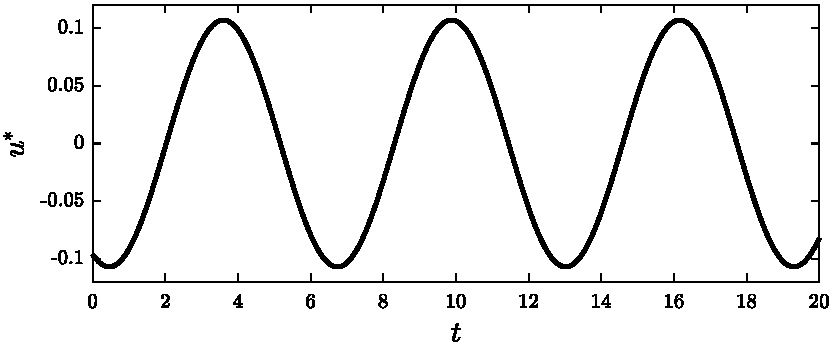
\includegraphics[width=\textwidth]{../ch5/figures/ex1sol-controls}%
\caption{Control.}
\label{fig:ch5:ex1sol:controls}
\end{subfigure}%
\begin{subfigure}{0.5\textwidth}
\centering
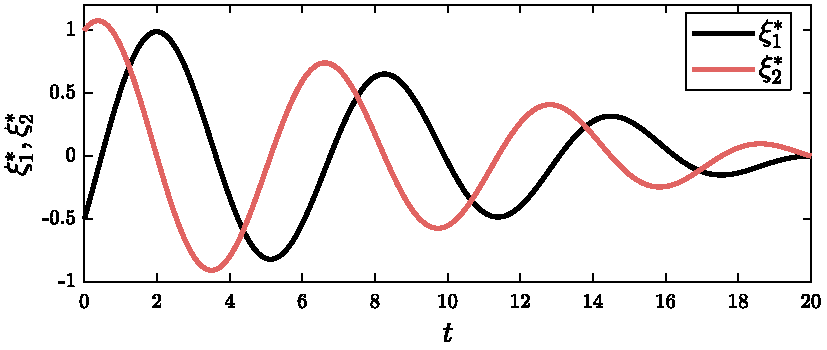
\includegraphics[width=\textwidth]{../ch5/figures/ex1sol-states}%
\caption{States.}
\label{fig:ch5:ex1sol:states}
\end{subfigure}%

\caption{Solution for \nameref{sec:ch5:example1}.}
\label{fig:ch5:ex1sol}
\end{figure}

It can be shown that the control trajectory that minimizes the objective while satisfying the constraints is:
\begin{align}
u^{\glsfoo[noindex]{optimal}}(t) = -\frac{2}{t_f^2 - \sin^2(t_f)}
\begin{bmatrix}
x_0 \\ v_0 
\end{bmatrix}\tran
\begin{bmatrix}
\sin(t_f -t) \sin(t_f) - t_f \sin(t) \\
-\cos(t_f -t) \sin(t_f) + t_f \cos(t)
\end{bmatrix}
\end{align}

\noindent with an optimal objective function value of:
\begin{align}
\Psi^* = \frac{t_f \left({v_{0}}^2+{x_{0}}^2\right)+2 {t_f}^2 v_{0} x_{0}-\cos\left(t_f\right) \sin\left(t_f\right) \left({v_{0}}^2-{x_{0}}^2\right)}{{{t_f}^2 - \sin\left(t_f\right)}^2} -2 v_{0} x_{0}
\end{align}

\noindent The problem parameters used are $t \in [0, 20]$, $x_0 = -1/2$, and $v_0 = 1$.
With these parameter values, $\Psi^* = 0.059842$.
The optimal trajectories for both the control and states is shown in Fig.~\ref{fig:ch5:ex1sol}.

%-------------------------------------------------------------
\subsubsection{Numerical Results}

% (convergence)
The convergence results for the eight tested schemes are shown in Fig.~\ref{fig:ch5:ex1sens:objective} (objective) and Fig.~\ref{fig:ch5:ex1sens:control} (controls).
The best scheme in terms of overall convergence rate was LGL-PS-G (7), and it is nearly linear.
However, once the scheme's accuracy was near machine epsilon, an accuracy threshold was reached and even started to slowly diverge (perhaps due to small errors in the calculation of the differentiation matrix, weights, etc.).
The next best scheme was CGL-PS-CC (8). 
It seemed to have a similar convergence rate as the other PS-based scheme, but it eventually achieves a sublinear rate of convergence until it reaches the precision threshold (for the objective value).

The SS-based schemes now remain. The best was ED-HS-CQHS (5), although ED-RK4-CQHS (6) was only slightly worse.
These are the two schemes that utilize the proposed CQHS quadrature method.
The convergence rate seemed to be sublinear, and an objective value accuracy threshold was reached for both schemes.
The control error between these schemes was nearly identical.
Next, perhaps surprisingly, was ED-ZOH-CEF (1).
Even though this scheme assumed piecewise constant control, it performed better than some of the more classical SS-based schemes.
Some of this accuracy may be due to the exact approximation of the objective function (i.e.,~only $u^2$ terms). 
ED-HS-CTR (4) was slightly better than ED-TR-CTR (3), indicating that the higher-order HS method did indeed provide additional accuracy for the same number of nodes.
Finally, ED-ZOH-CEF (1) was the worst scheme tested.

\begin{figure}%
\centering

{\footnotesize Local maximum values (local minimum values are in a thinner, translucent color):}


\includegraphics[width=\textwidth]{../ch5/figures/ex1_sens_legend}%

\vspace{1mm}

\begin{subfigure}{0.5\textwidth}
\centering
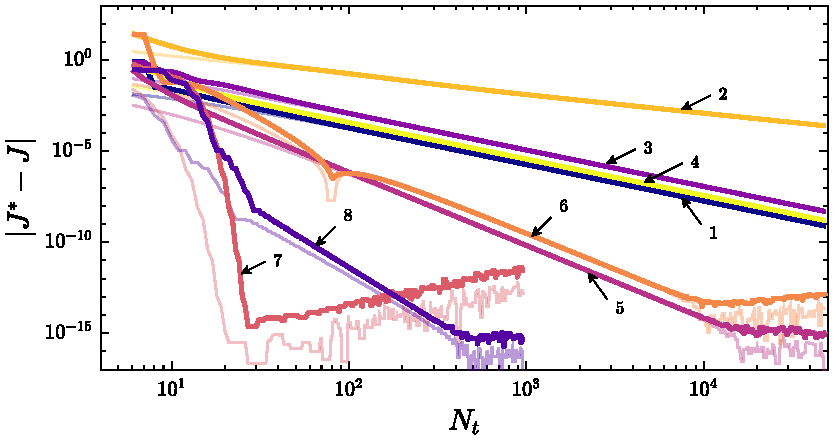
\includegraphics[width=\textwidth]{../ch5/figures/ex1_sens_objective}%
\caption{Objective error.}
\label{fig:ch5:ex1sens:objective}
\end{subfigure}%
\begin{subfigure}{0.5\textwidth}
\centering
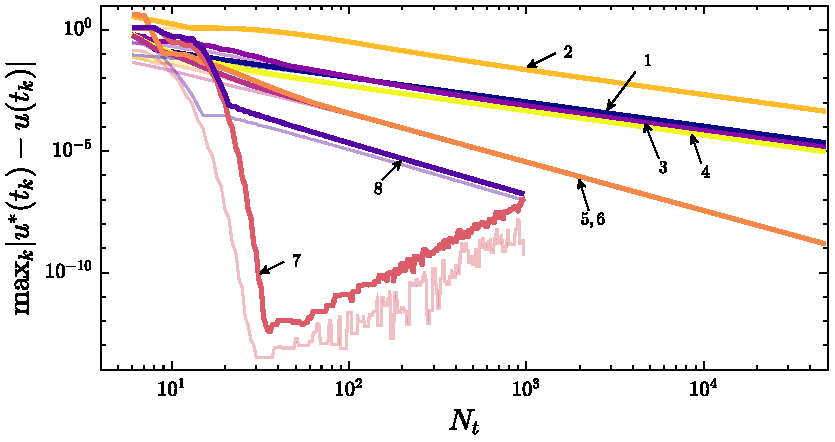
\includegraphics[width=\textwidth]{../ch5/figures/ex1_sens_control}%
\caption{Control error.}
\label{fig:ch5:ex1sens:control}
\end{subfigure}%

\begin{subfigure}{0.5\textwidth}
\centering
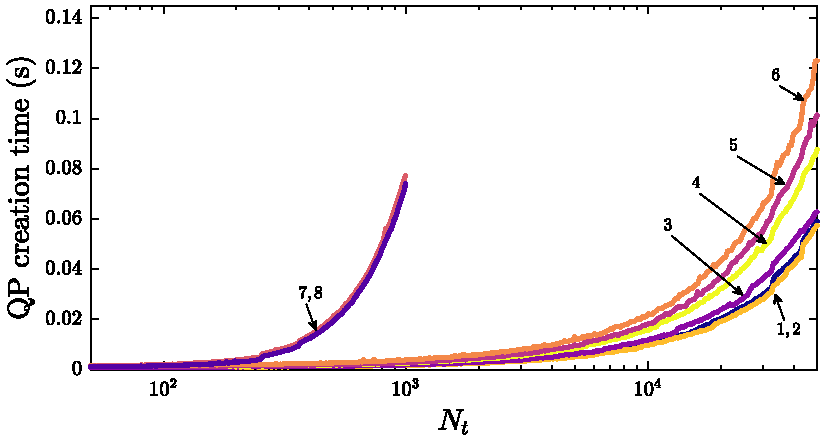
\includegraphics[width=\textwidth]{../ch5/figures/ex1_sens_qp_time}%
\caption{\qp{} creation time vs. $N_t$.}
\label{fig:ch5:ex1sens:qptime}
\end{subfigure}%
\begin{subfigure}{0.5\textwidth}
\centering
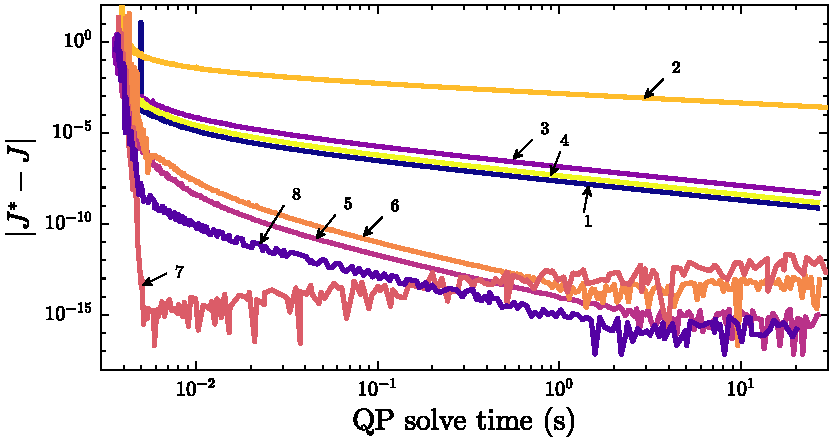
\includegraphics[width=\textwidth]{../ch5/figures/ex1_sens_solve_time}%
\caption{Objective error vs. total \qp{} solve time.}
\label{fig:ch5:ex1sens:solvetime}
\end{subfigure}%

\caption{Numerical results for \nameref{sec:ch5:example1}.}
\label{fig:ch5:ex1sens}
\end{figure}%

% new paragraph (qp creation time)
The time to create the \qp{} vs.~$N_t$ for each scheme is shown in Fig.~\ref{fig:ch5:ex1sens:qptime}.
Here we see two distinct groups: one for the PS-based schemes, and one for the SS-based schemes.
The PS-based schemes take a longer amount of time for a specific $N_t$ because the sparse matrices are much denser (cf. Fig.~\ref{fig:figsparsityAPS} and Fig.~\ref{fig:figsparsityASS}).
The primary cost is the construction of the sparse matrices from the sequences.
The SS-based schemes do vary in their creation time with the schemes, with more matrix calculations and denser defect constraint matrices being slower to create.
Therefore, we observe that (1) is the fastest and (6) is the slowest.
All creation times for this problem are under 0.13~s, even for larger $N_t$.

% new paragraph (qp solve time)
A fairer comparison between the schemes considers the tradeoffs between accuracy and total solve time.
The time to create and solve the \qp{} vs. the error in the objective function is shown in Fig.~\ref{fig:ch5:ex1sens:solvetime}.
The ordering is generally the same as the error plots, and (7) is clearly the preferred scheme for this problem.
Schemes (5) and (6) are slightly more attractive as the computation time for a given error is only slightly slower than the PS-based schemes.

%-------------------------------------------------------------
\subsection{Example 2} \label{sec:ch5:example2}

%-------------------------------------------------------------
\subsubsection{Description}
For the second example, we will consider the problem on pp.~120--122 from Ref.~\cite{Bryson1975a} and in Ref.~\cite{Bryson1963a}:
\begin{subequations}%%
\begin{align}
\min_{u} \quad & \frac{1}{2}\int_{0}^{1} u^2 dt \\
\text{subject to:} \quad  & \dot{\bm{\xi}} = \begin{bmatrix} \xi_2 \\ u \end{bmatrix} \\
& \xi_1(0) = 0, \quad \xi_1(1) = 0, \quad \xi_2(0) = 1, \quad \xi_2(1) = -1 \\
& \xi_1(t) \leq \ell
\end{align}
\end{subequations}%

\noindent This problem is similar to \nameref{sec:ch5:example1} but, now has a path constraint.
The structure-based problem description for this example is:%
\allowdisplaybreaks[1]
\begin{subequations}%
\begin{gather}
% Lagrange term
\mathcal{L}\xind{1}.\xvar{left} = 1, \quad \mathcal{L}\xind{1}.\xvar{right} = 1, \quad \mathcal{L}\xind{1}.\xvar{matrix} = 1/2 \\
% system dynamics
\bm{A} = \begin{bmatrix} 0 & 1 \\ 0 & 0
\end{bmatrix}, \quad \bm{B} = \begin{bmatrix} 0 \\ 1
\end{bmatrix} \\
% linear equality constraints
\mathcal{LB}\xind{1}.\xvar{right} = 4, \quad \mathcal{LB}\xind{1}.\xvar{matrix} = \begin{bmatrix} 0 & 1 \end{bmatrix}\tran \\
\mathcal{LB}\xind{2}.\xvar{right} = 5, \quad \mathcal{LB}\xind{2}.\xvar{matrix} = \begin{bmatrix} 0 & -1 \end{bmatrix}\tran \\
\mathcal{UB}\xind{1}.\xvar{right} = 4, \quad \mathcal{UB}\xind{1}.\xvar{matrix} = \begin{bmatrix} 0 & 1 \end{bmatrix}\tran \\
\mathcal{UB}\xind{2}.\xvar{right} = 5, \quad \mathcal{UB}\xind{2}.\xvar{matrix} = \begin{bmatrix} 0 & -1 \end{bmatrix}\tran \\
\mathcal{UB}\xind{3}.\xvar{right} = 2, \quad \mathcal{UB}\xind{3}.\xvar{matrix} = \begin{bmatrix}\ell & \infty \end{bmatrix}\tran % \\
\end{gather}
\end{subequations}%%
\allowdisplaybreaks[0]%

\noindent The \textsc{Matlab} code is in Sec.~\ref{sec:ex2-code}.

%-------------------------------------------------------------
\subsubsection{Solution}

\begin{figure}
\centering

\begin{subfigure}{0.5\textwidth}
\centering
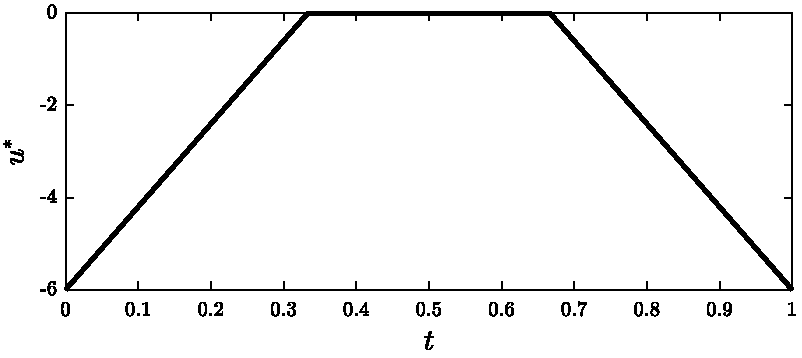
\includegraphics[width=\textwidth]{../ch5/figures/ex2sol-controls}%
\caption{Control.}
\label{fig:ch5:ex2sol:controls}
\end{subfigure}%
\begin{subfigure}{0.5\textwidth}
\centering
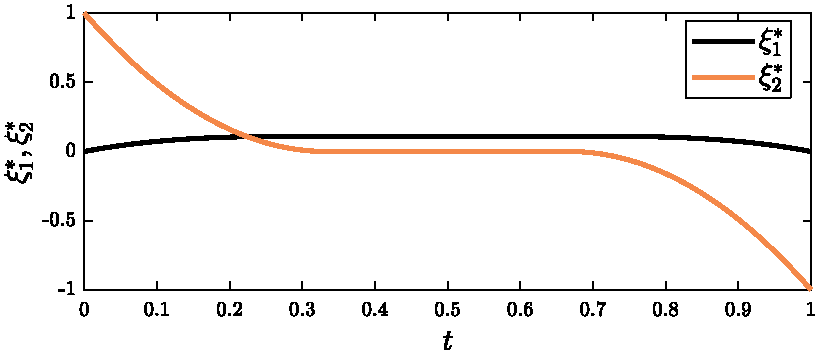
\includegraphics[width=\textwidth]{../ch5/figures/ex2sol-states}%
\caption{States.}
\label{fig:ch5:ex2sol:states}
\end{subfigure}%

\caption{Solution for \nameref{sec:ch5:example2}.}
\label{fig:ch5:ex2sol}
\end{figure}

It can be shown that the control trajectory that minimizes the objective while satisfying the constraints when $0 < \ell \leq 1/6$ is:
\begin{align}
u^*(t) = \begin{cases}
-\frac{2}{3\ell}\left( 1 - \frac{t}{3\ell} \right) & 0 \leq t < 3\ell \\
0 & 3\ell \leq t < 1 - 3\ell \\
-\frac{2}{3\ell}\left( 1 - \frac{1-t}{3\ell} \right) & 0 \leq t \leq 3\ell \\
\end{cases}
\end{align}

\noindent with an optimal objective function value of:
\begin{align}
\Psi^* = \frac{4}{9\ell}
\end{align}

\noindent A problem parameter value of $\ell = 1/9$ will be used, and with this value, $\Psi^* = 4$.
The optimal trajectories for both the control and states are shown in Fig.~\ref{fig:ch5:ex2sol}.

%-------------------------------------------------------------
\subsubsection{Numerical Results}

The convergence results for the eight tested schemes are shown in Fig.~\ref{fig:ch5:ex2sens}.
All schemes, including the PS-based schemes, achieve similar sublinear convergence rates, and this is due to the path constraint.
For the ED meshes, if $N_t-1$ was a multiple of 3, then nodes values of $1/3$ and $2/3$ would be directly included in the mesh.
Otherwise, the locations where the path constraint changes activity (in the true solution) would not be included.
Therefore, there is slow convergence due to errors around these points.
However, when $N_t=4$ with ED-HS-CQHS (5) or ED-RK4-CQHS (6), all relevant quantities (states, control, and objective value) are accurate within the machine precision!
Such accuracy with a minimal number of node points was previously only possible with specifically constructed multiple-interval PS methods \cite{Herber2015a}.
Since the optimal control policy is piecewise linear, the CQHS method is exactly accurate for $u^2$ terms.
Furthermore, the states are piecewise quadratic and cubic and both the HS and RK4 methods exactly approximate these dynamics.
Therefore, schemes (5,6) exactly represent the original problem.

% new paragraph
Ignoring the favorable meshes and looking at the local worst errors, we still see (5,6) performing the best along with ED-ZOH-CEF (1) (except with respect to the controls).
These are followed closely by the other methods except for ED-EF-CEF (2), which was the worst method again.
These results for the PS-based schemes demonstrate the potentially issue with using a single global polynomial when path constraints are present \cite{Darby2009a, Darby2011a}.
Multiple-interval PS methods would be more suitable for this type of problem (see Sec.~\ref{sec:ch5:multipleinterval}).

\begin{figure}%
\centering

{\footnotesize Local maximum values (local minimum values are in a thinner, translucent color):}


\includegraphics[width=\textwidth]{../ch5/figures/ex1_sens_legend}%

\vspace{1mm}

\begin{subfigure}{0.5\textwidth}
\centering
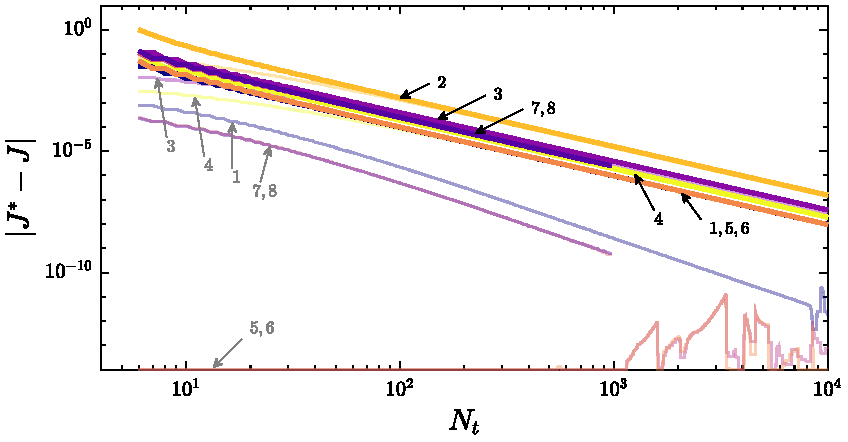
\includegraphics[width=\textwidth]{../ch5/figures/ex2_sens_objective}%
\caption{Objective error.}
\label{fig:ch5:ex2sens:objective}
\end{subfigure}%
\begin{subfigure}{0.5\textwidth}
\centering
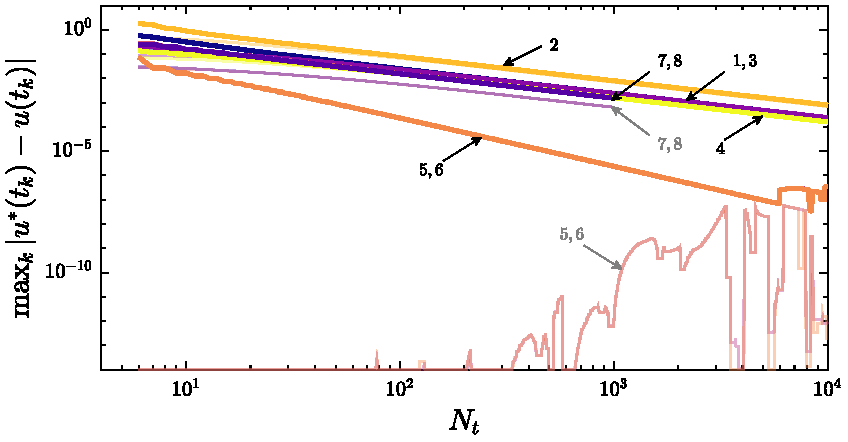
\includegraphics[width=\textwidth]{../ch5/figures/ex2_sens_control}%
\caption{Control error.}
\label{fig:ch5:ex2sens:control}
\end{subfigure}%

\begin{subfigure}{0.5\textwidth}
\centering
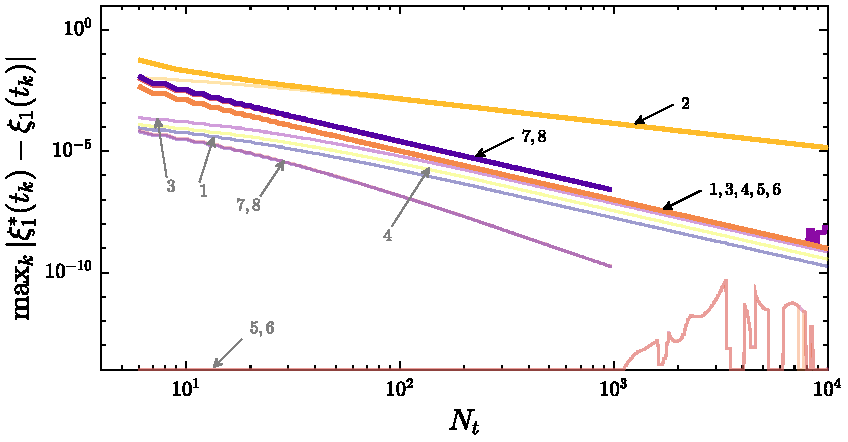
\includegraphics[width=\textwidth]{../ch5/figures/ex2_sens_state_1}%
\caption{$\xi_1$ error.}
\label{fig:ch5:ex2sens:state:1}
\end{subfigure}%
\begin{subfigure}{0.5\textwidth}
\centering
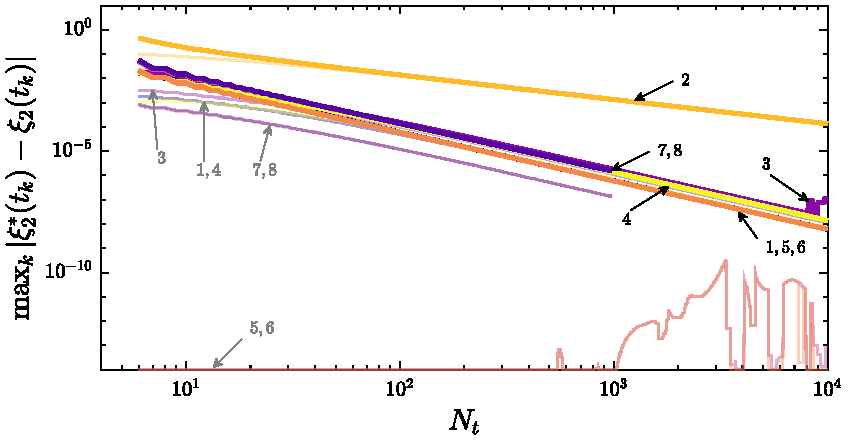
\includegraphics[width=\textwidth]{../ch5/figures/ex2_sens_state_2}%
\caption{$\xi_2$ error.}
\label{fig:ch5:ex2sens:state:2}
\end{subfigure}%

\caption{Numerical results for \nameref{sec:ch5:example2}.}
\label{fig:ch5:ex2sens}
\end{figure}

%-------------------------------------------------------------
\subsection{Example 3} \label{sec:ch5:example3}

%-------------------------------------------------------------
\subsubsection{Description}

For the third example, we will consider the problem on pp.~109--110 of Ref.~\cite{Bryson1975a}:
\begin{subequations}%%
\begin{align}
\min_{u(t)} \quad & \frac{a^2}{2} [ \xi(t_f) ]^2 + \frac{1}{2}\int_{0}^{t_f} u^2 dt \\
\text{subject to:} \quad  & \dot{\xi} = b(t) u \\
& \xi(0) = \xi_0 \\
& \abs{u(t)} \leq 1
\end{align}
\end{subequations}%

\noindent This problem has time-varying matrices, path constraints, and both Lagrange and Mayer terms.
The structure-based problem description for this example is:
\allowdisplaybreaks[1]%
\begin{subequations}%%
\begin{gather}
% Mayer term
\mathcal{M}\xind{1}.\xvar{left} = 5, \quad \mathcal{M}\xind{1}.\xvar{right} = 5, \quad \mathcal{M}\xind{1}.\xvar{matrix} = a^2/2 \\
% Lagrange term
\mathcal{L}\xind{1}.\xvar{left} = 1, \quad \mathcal{L}\xind{1}.\xvar{right} = 1, \quad \mathcal{L}\xind{1}.\xvar{matrix} = 1/2 \\
% dynamics
A = 0, \quad B = b(t) \\
% initial condition
% simple bound
\mathcal{UB}\xind{1}.\xvar{right} = 4, \quad \mathcal{UB}\xind{1}.\xvar{matrix} = \xi_0, \quad
\mathcal{LB}\xind{1}.\xvar{right} = 4, \quad \mathcal{LB}\xind{1}.\xvar{matrix} = \xi_0 \\
\mathcal{UB}\xind{2}.\xvar{right} = 1, \quad \mathcal{UB}\xind{2}.\xvar{matrix} = 1, \quad
\mathcal{LB}\xind{2}.\xvar{right} = 1, \quad \mathcal{LB}\xind{2}.\xvar{matrix} = -1
\end{gather}
\end{subequations}%%
\allowdisplaybreaks[0]%

\noindent The \textsc{Matlab} code is in Sec.~\ref{sec:ex3-code}.

%-------------------------------------------------------------
\subsubsection{Solution}

\begin{figure}
\centering

\begin{subfigure}{0.5\textwidth}
\centering
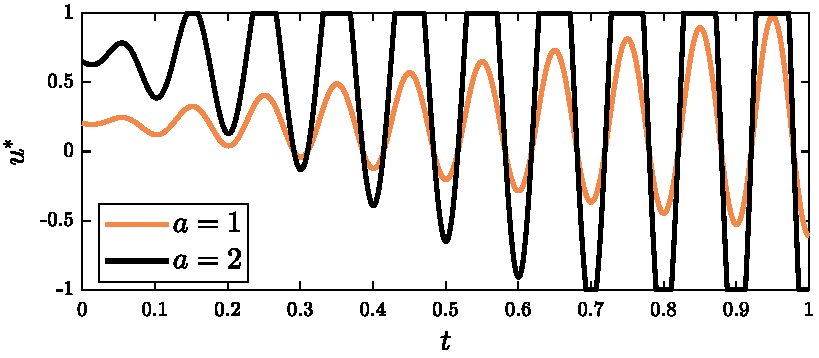
\includegraphics[width=\textwidth]{../ch5/figures/ex3sol-controls}%
\caption{Control.}
\label{fig:ch5:ex3sol:controls}
\end{subfigure}%
\begin{subfigure}{0.5\textwidth}
\centering
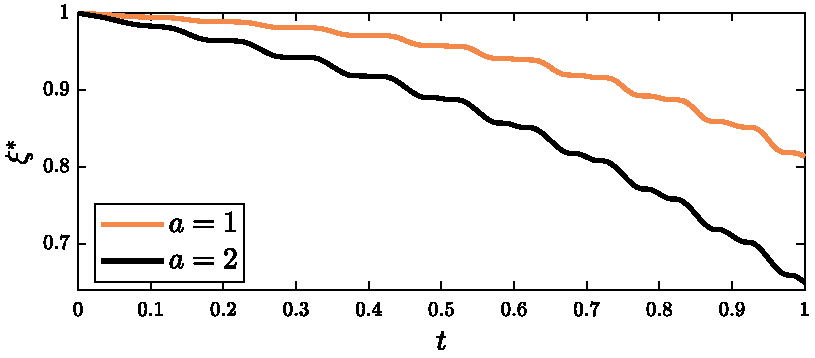
\includegraphics[width=\textwidth]{../ch5/figures/ex3sol-states}%
\caption{State.}
\label{fig:ch5:ex3sol:states}
\end{subfigure}%

\caption{Solutions for \nameref{sec:ch5:example3}.}
\label{fig:ch5:ex3sol}
\end{figure}

The optimal control is:
\begin{align}
u^*(t) &= - \mathrm{sat}\left[ a^2 b(t) \xi(t_f) \right]
\end{align}

\noindent where $\xi(t_f)$ is computed from the implication equation:
\begin{align}
\xi(t_f) &= \xi_0 - \int_0^{t_f} b(t) \mathrm{sat}\left[ a^2 b(t) \xi(t_f) \right] dt 
\end{align}

\noindent The problem parameters used are $t_f = 1$, $\xi_0 = 1$, and $b(t) = t \cos(20 \pi t) - 1/4$.
Both $a = 1$ and $a = 2$ will be tested.
For $a=1$, $\Psi^* = 0.406759$ and $\xi^*(t_f) = 0.813517$.
For $a=2$, $\Psi^* = 1.150647$ and $\xi^*(t_f) = 0.649528$.
The optimal trajectories for control and state for both values of $a$ are shown in Fig.~\ref{fig:ch5:ex3sol}.
With $a=1$, the path constraints are never active, but with $a=2$, the path constraints switch activity frequently. 

%-------------------------------------------------------------
\subsubsection{Numerical Results}

\begin{figure}%
\centering

{\footnotesize Local maximum values (local minimum values are in a thinner, translucent color):}


\includegraphics[width=\textwidth]{../ch5/figures/ex1_sens_legend}%

\vspace{1mm}

\begin{subfigure}{0.5\textwidth}
\centering
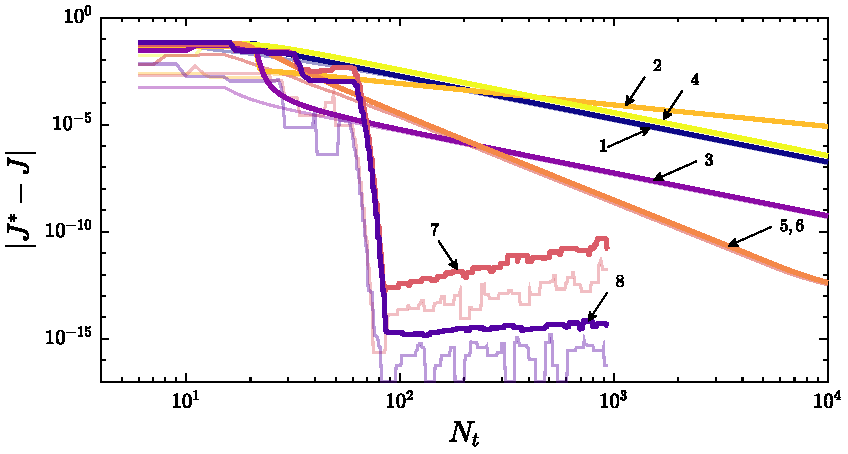
\includegraphics[width=\textwidth]{../ch5/figures/ex3_sens_objective_a1}%
\caption{Objective error with $a=1$.}
\label{fig:ch5:ex3sens:objective:a1}
\end{subfigure}%
\begin{subfigure}{0.5\textwidth}
\centering
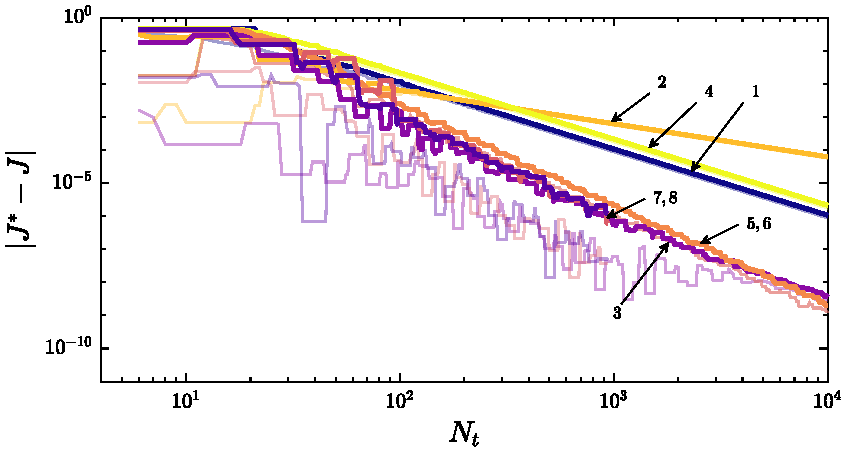
\includegraphics[width=\textwidth]{../ch5/figures/ex3_sens_objective_a2}%
\caption{Objective error with $a=2$.}
\label{fig:ch5:ex3sens:objective:a2}
\end{subfigure}%

\begin{subfigure}{0.5\textwidth}
\centering
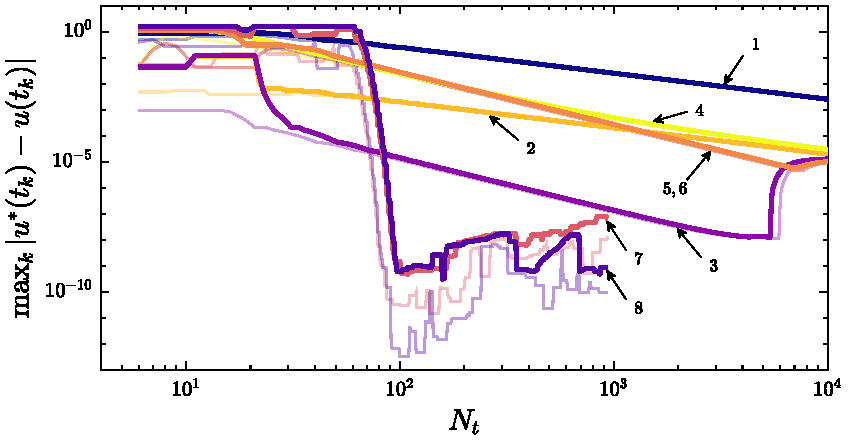
\includegraphics[width=\textwidth]{../ch5/figures/ex3_sens_control_a1}%
\caption{Control error with $a=1$.}
\label{fig:ch5:ex3sens:control:a1}
\end{subfigure}%
\begin{subfigure}{0.5\textwidth}
\centering
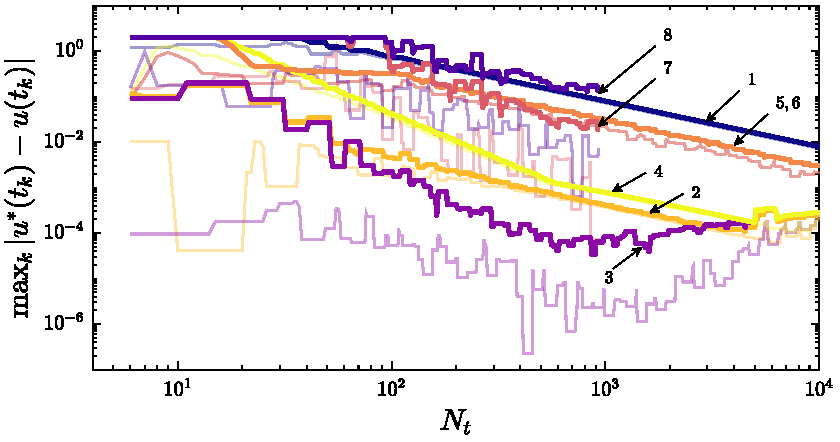
\includegraphics[width=\textwidth]{../ch5/figures/ex3_sens_control_a2}%
\caption{Control error with $a=2$.}
\label{fig:ch5:ex3sens:control:a2}
\end{subfigure}%

\begin{subfigure}{0.5\textwidth}
\centering
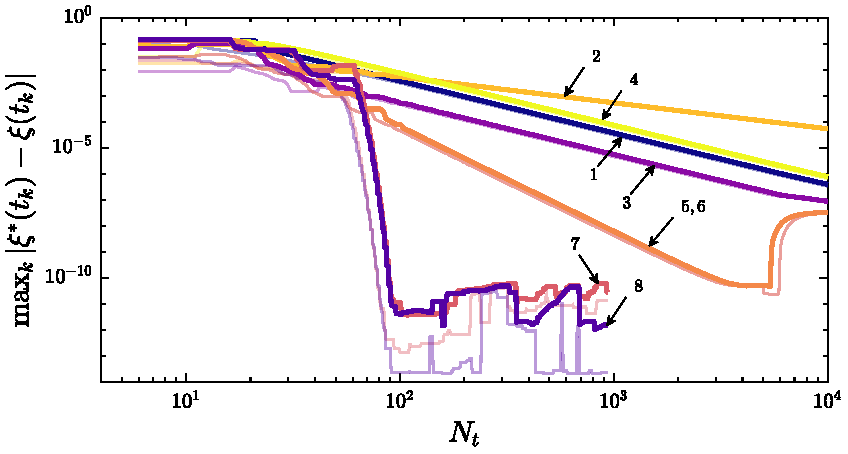
\includegraphics[width=\textwidth]{../ch5/figures/ex3_sens_state_1_a1}%
\caption{State error with $a=1$.}
\label{fig:ch5:ex3sens:state:a1}
\end{subfigure}%
\begin{subfigure}{0.5\textwidth}
\centering
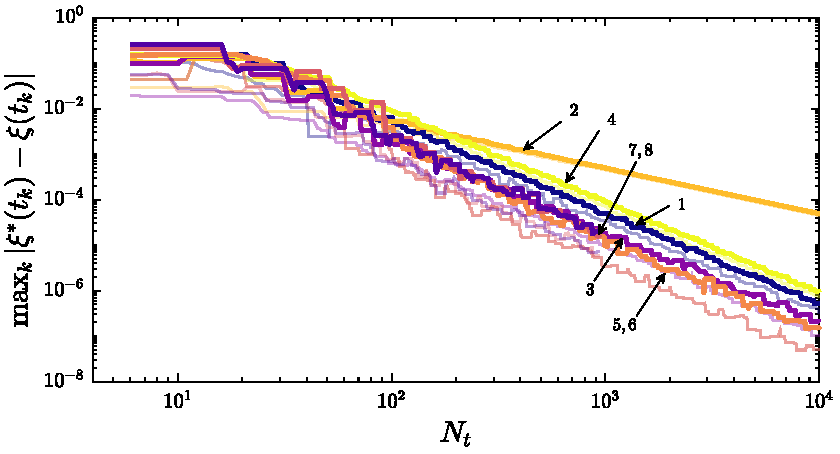
\includegraphics[width=\textwidth]{../ch5/figures/ex3_sens_state_1_a2}%
\caption{State error with $a=2$.}
\label{fig:ch5:ex3sens:state:a2}
\end{subfigure}%

\caption{Numerical results for \nameref{sec:ch5:example3}.}
\label{fig:ch5:ex3sens}
\end{figure}

The convergence results for the eight tested schemes and both values of $a$ are shown in Fig.~\ref{fig:ch5:ex3sens}.
When $a=1$ (where the path constraints are not active), the results are somewhat similar to \nameref{sec:ch5:example1}.
The best methods are the two PS-based schemes (7,8), but unlike the previous example, the gap between them is negligible.
Although the SS-based schemes are converging to the true solution, the ranking of the schemes depends highly on the relative preference between the objective, control, or state errors.
The two CQHS-based schemes have lower state error, but higher control error.
ED-TR-CTR (3) has much lower control error, but higher state error. 
With respect to the objective error, (3) begins with lower error but there is a transition point around $N_t=200$ where (5,6) exhibit less error.
We also see ED-HS-CTR (4) performing worse than (3), differing from the previous examples.

% new paragraph
With $a=2$, the results are quite different with more sporadic convergence behavior (especially for the control).
We observe that (3) is now the best scheme.
Combining the results from both values of $a$, (3) appears to be the best option if high accuracy is required in both problem versions.
These unexpected results might be explained by the fact that there is no $\bm{A}$ in this example (a fairly uncommon property in \lqdo). As a result, this example may prove to be a useful, challenging test problem in the future.
As a result, this example may prove to be a useful, challenging test problem in the future.
Fully understanding these results is left as future work.

%-------------------------------------------------------------
\subsection{Example 4} \label{sec:ch5:example4}

%-------------------------------------------------------------
\subsubsection{Description}

For the fourth example, we will consider the finite-horizon LQR problem in Prob.~(\ref{eq:ch5:lqr}) \cite{Bryson1975a,Liberzon2012a}:%
\begin{subequations}%%
\begin{align}
\min_{\bm{u}(t)} \quad & \left[ \bm{\xi}\tran \bm{M} \bm{\xi} \right]_{t=t_f} + 
\int_{t_0}^{t_f} \left[ \bm{\xi}\tran \bm{Q} \bm{\xi} + \bm{u}\tran \bm{R} \bm{u} \right] dt \\
\text{subject to:} \quad & \dot{\bm{\xi}} = \bm{A} \bm{\xi} + \bm{B} \bm{u} \\
& \bm{\xi}(t_0) = \bm{\xi}_0
\end{align}
\end{subequations}%

\noindent where $\bm{M}$ and $\bm{Q}$ are symmetric positive semidefinite and $\bm{R}$ is symmetric positive definite.
The structure-based problem description for this example is:%
\allowdisplaybreaks[1]%
\begin{subequations}%%
\begin{gather}
% Mayer term
\mathcal{M}\xind{1}.\xvar{left} = 5, \quad \mathcal{M}\xind{1}.\xvar{right} = 5, \quad \mathcal{M}\xind{1}.\xvar{matrix} = \bm{M} \\
% Lagrange term
\mathcal{L}\xind{1}.\xvar{left} = 2, \quad \mathcal{L}\xind{1}.\xvar{right} = 2, \quad \mathcal{L}\xind{1}.\xvar{matrix} = \bm{Q} \\
\mathcal{L}\xind{2}.\xvar{left} = 1, \quad \mathcal{L}\xind{2}.\xvar{right} = 1, \quad \mathcal{L}\xind{2}.\xvar{matrix} = \bm{R} \\
% dynamics
% \bm{A}, \bm{B} \text{ given} \\
% initial condition
\mathcal{UB}\xind{1}.\xvar{right} = 4, \quad \mathcal{UB}\xind{1}.\xvar{matrix} = \bm{\xi}_0, \quad
\mathcal{LB}\xind{1}.\xvar{right} = 4, \quad \mathcal{LB}\xind{1}.\xvar{matrix} = \bm{\xi}_0
\end{gather}
\end{subequations}%%
\allowdisplaybreaks[0]%

\noindent The \textsc{Matlab} code is in Sec.~\ref{sec:ex4-code}.

%-------------------------------------------------------------
\subsubsection{Solution} \label{sec:ch5:ex4:solution}

\begin{figure}
\centering

\begin{subfigure}{0.5\textwidth}
\centering
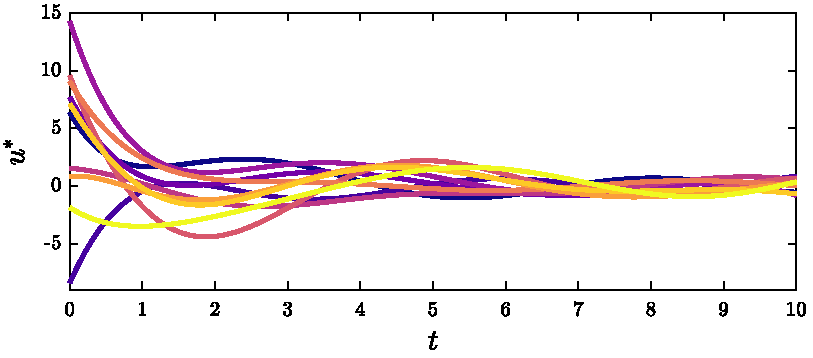
\includegraphics[width=\textwidth]{../ch5/figures/ex4sol-controls}%
\caption{Control.}
\label{fig:ch5:ex4sol:controls}
\end{subfigure}%
\begin{subfigure}{0.5\textwidth}
\centering
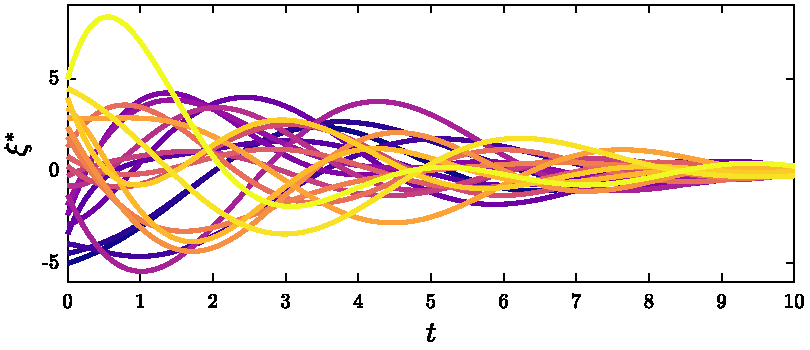
\includegraphics[width=\textwidth]{../ch5/figures/ex4sol-states}%
\caption{States.}
\label{fig:ch5:ex4sol:states}
\end{subfigure}%

\caption{Solution for \nameref{sec:ch5:example4}.}
\label{fig:ch5:ex4sol}
\end{figure}

The optimal control has the following form \cite{Bryson1975a,Liberzon2012a}:
\begin{align}
\bm{u}^* = - \bm{R}^{-1} \bm{B}\tran \bm{P} \bm{\xi}
\end{align}

\noindent where $\bm{P}$ is symmetric positive semidefinite matrix that is a solution to the following differential equation and boundary condition:
\begin{align}
\dot{\bm{P}} = -\bm{Q} - \bm{A}\tran \bm{P} - \bm{P} \bm{A} + \bm{P} \bm{B} \bm{R}^{-1} \bm{B}\tran \bm{P}, \quad \bm{P}(t_f) = \bm{M}
\end{align}

\noindent The specific problem parameters are shown in Sec.~\ref{sec:ex4-code} ($n_\xi = 20$ and $n_u=10$ with generated matrices).
The optimal trajectories for controls and states are shown in Fig.~\ref{fig:ch5:ex4sol}, and were determined by numerically solving the BVP problem with a relative error tolerance at $10^{-10}$.

%-------------------------------------------------------------
\subsubsection{Numerical results}

\begin{figure}%
\centering

{\footnotesize Local maximum values (local minimum values are in a thinner, translucent color):}


\includegraphics[width=\textwidth]{../ch5/figures/ex1_sens_legend}%

\vspace{1mm}

\begin{subfigure}{0.5\textwidth}
\centering
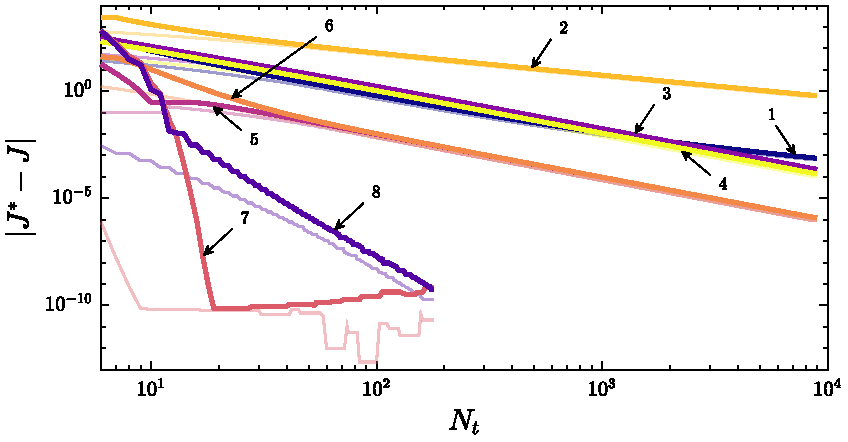
\includegraphics[width=\textwidth]{../ch5/figures/ex4_sens_objective}%
\caption{Objective error.}
\label{fig:ch5:ex4sens:objective}
\end{subfigure}%
\begin{subfigure}{0.5\textwidth}
\centering
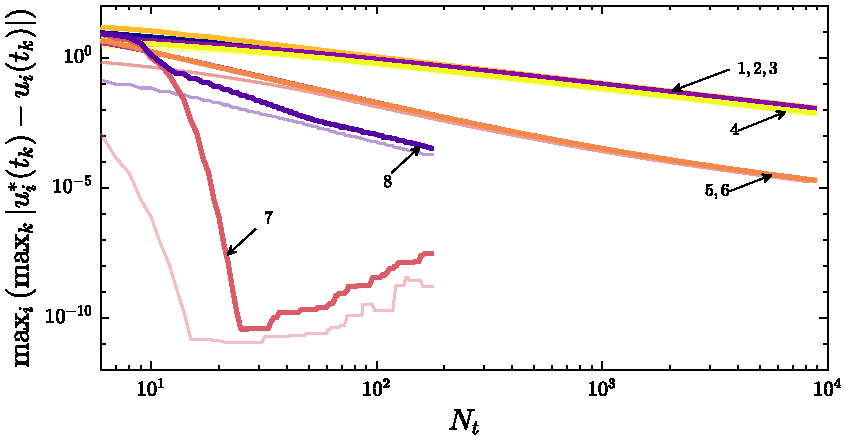
\includegraphics[width=\textwidth]{../ch5/figures/ex4_sens_control}%
\caption{Control error.}
\label{fig:ch5:ex4sens:control}
\end{subfigure}%

\begin{subfigure}{0.5\textwidth}
\centering
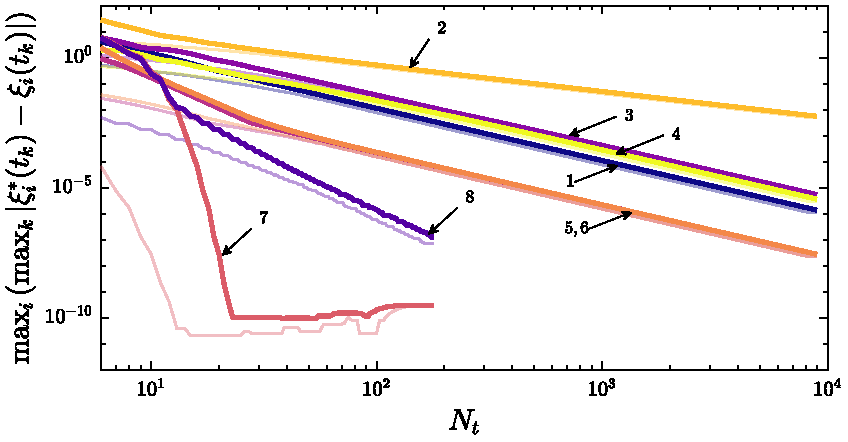
\includegraphics[width=\textwidth]{../ch5/figures/ex4_sens_state_1}%
\caption{State error.}
\label{fig:ch5:ex4sens:state-1}
\end{subfigure}%
\begin{subfigure}{0.5\textwidth}
\centering
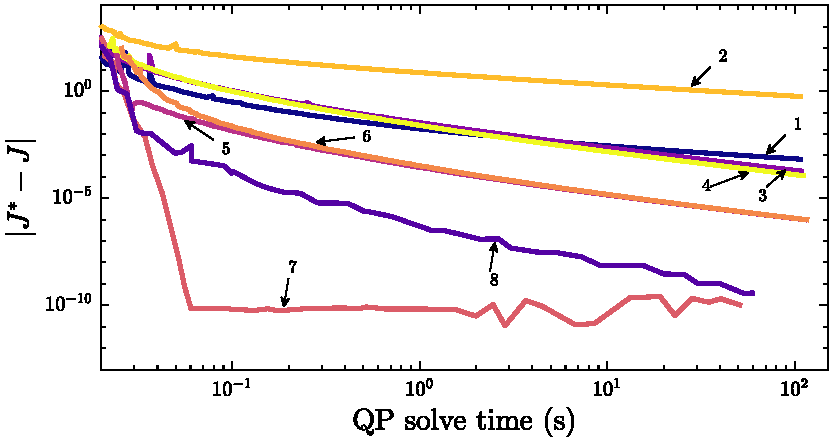
\includegraphics[width=\textwidth]{../ch5/figures/ex4_sens_solve_time}%
\caption{Objective error vs. total \qp{} solve time.}
\label{fig:ch5:ex4sens:solvetime}
\end{subfigure}%

\caption{Numerical results for \nameref{sec:ch5:example4}.}
\label{fig:ch5:ex4sens}
\end{figure}

The convergence results for the eight tested schemes are shown in Fig.~\ref{fig:ch5:ex4sens}.
The numerical results for this example are quite similar to \nameref{sec:ch5:example1} (see Fig.~\ref{fig:ch5:ex1sens}).
The PS-based methods (7,8) performed the best, followed by the CQHS-based methods (5,6). Then was (1,3,4) and finally (1) was the worst again.
The primary discussion point for this example is the efficiency at which the LQR problem was solved.
The objective error vs. total \qp{} solve time is shown in Fig.~\ref{fig:ch5:ex4sens:solvetime}.
LGL-PS-G (7) with $N_t=23$ took only 0.2~s to create and solve the \qp{} with an accuracy in states, controls, and objective value at the tolerance used ($10^{-10}$) when generating the BVP solution in Sec.~\ref{sec:ch5:ex4:solution}.
These results demonstrate that \dt{} approximations of the finite-horizon LQR problem can be a competitive solution strategy.

%-------------------------------------------------------------
\subsection{Example 5} \label{sec:ch5:example5}

%-------------------------------------------------------------
\subsubsection{Description}

The final example is a constructed problem that will help demonstrate some of the problem elements and extensions in Sec.~\ref{sec:ch5:extensions} not seen in the previous examples.
The infinite-dimensional problem formulation is:%
\allowdisplaybreaks[1]%
\begin{subequations}%%
\begin{align}
\min_{\bm{u}(t)} \quad & \int_0^1 \left[ u_1^2/10 + u_2^2/10 + u_1\xi_1 + u_1\xi_2 + 5\left(\xi_2-g(t)\right)^2 \right] dt + \max_{0\leq t\leq 1} \xi_3(t) \\
\text{subject to:} \quad & \dot{\bm{\xi}} = \begin{bmatrix} -1 & 2 & 0 \\ 3 & -4 & 0 \\ 1 & 2 & -1 \end{bmatrix} \bm{\xi} +
\begin{bmatrix} 1 & 0 \\ -1 & 0 \\ 0 & 1/20 \end{bmatrix} \bm{u} \\
& \xi_1(0) = 2, \quad \xi_3(0) = 1/2 \\
& \xi_2(0) - \xi_2(1) = 0 \\
& \int_0^1 \xi_1(t) dt = 0 \\
& -\xi_1(t) + u_2(t)/12 \leq 0 \\
& \xi_2(t) \leq g(t) \\
& \abs{u_2} \leq 10 
\end{align}
\end{subequations}%%
\allowdisplaybreaks[0]%

\noindent where 
$5\left(\xi_2-g(t)\right)^2$ is an output tracking term (resulting in time-varying quadratic, linear, and constant objective function terms, see Sec.~\ref{sec:ch5:output}),
$\max\xi_3(t)$ is a min-max objective term (that will be approximated with a parameter, see Sec.~\ref{sec:ch5:minmax:objective}),
$\xi_2(0) - \xi_2(1) = 0$ is a periodic constraint (that will be implemented as a linear equality constraint),
$\int_0^1 \xi_1(t) dt = 0$ is an integral constraint (which will be approximated with an additional state, see Sec.~\ref{sec:ch5:integral:constraints}),
$-\xi_1(t) + u_2(t)/12 \leq 0$ is a mixed control-state path constraint,
$\xi_2(t) \leq g(t) $ is a time-varying simple bound,
and
$\abs{u_2} \leq 10 $ is a linear absolute value constraint (that will be implemented with two constraints, see Sec.~\ref{sec:ch5:absolute:values}).
For brevity, the structure-based implementation is only shown in the \textsc{Matlab} code in Sec.~\ref{sec:ex5-code}. 

%-------------------------------------------------------------
\subsubsection{Solution}

This example, like many \lqdo{} problems, does not have a straightforward solution, so we can instead use \dt{} to obtain an approximate solution.
Here we set $g(t) = \sin(2 \pi t) +1/2$.
The optimal trajectories for the states and controls are shown in Fig.~\ref{fig:ch5:ex5sens} along with the trajectories for the integral and mixed control-state constraints.
This solution was found using ED-HS-CQHS (5) with 5,000 node points and $\Psi^*=6.368153$.
All constraints are satisfied, and all the path constraints enter and exit activity during the time horizon.

\begin{figure}
\centering

\begin{subfigure}{0.5\textwidth}
\centering
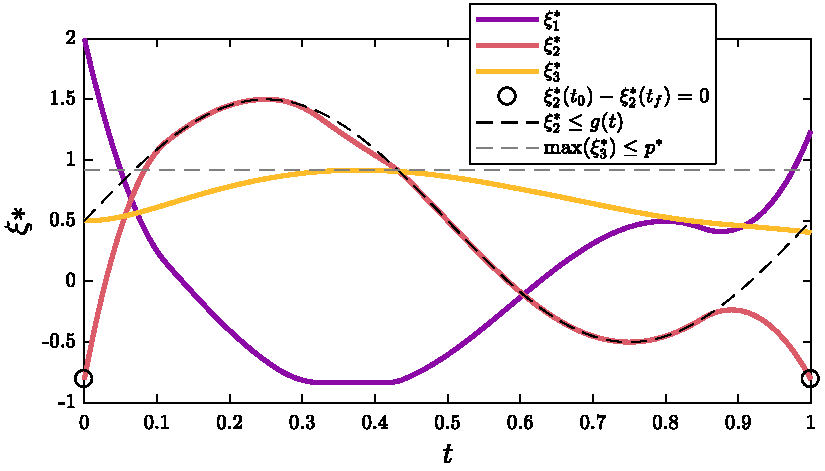
\includegraphics[width=\textwidth]{../ch5/figures/ex5sol-states}%
\caption{States.}
\label{fig:ch5:ex5sol:states}
\end{subfigure}%
\begin{subfigure}{0.5\textwidth}
\centering
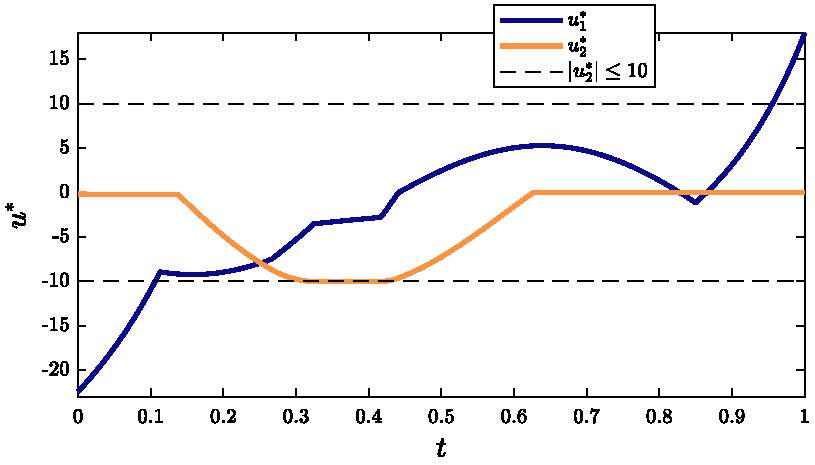
\includegraphics[width=\textwidth]{../ch5/figures/ex5sol-controls}%
\caption{Controls.}
\label{fig:ch5:ex5sol:controls}
\end{subfigure}%

\begin{subfigure}{\textwidth}
\centering
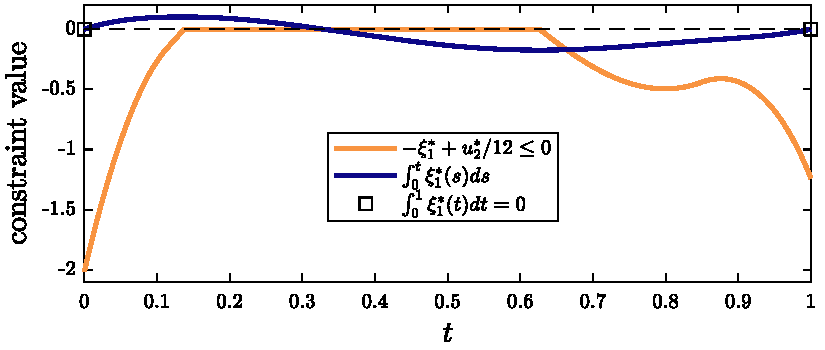
\includegraphics[width=0.5\textwidth]{../ch5/figures/ex5sol-other}%
\caption{Integral and mixed state-control path constraints.}
\label{fig:ch5:ex5sol:other}
\end{subfigure}%

\caption{Solution for \nameref{sec:ch5:example5}.}
\label{fig:ch5:ex5sens}
\end{figure}